\documentclass[reqno,12pt,notitlepage]{article}
\usepackage{amsmath}
\usepackage{amsthm}
\usepackage{amssymb}
\usepackage{setspace}
\usepackage{graphicx}
\usepackage{booktabs}
\usepackage{pdflscape}
\usepackage{url}
\usepackage{caption}
\usepackage{multirow,rotating,multicol}
\usepackage{listings}
\usepackage[bookmarks,hidelinks]{hyperref}
\usepackage{longtable}
\usepackage{threeparttable}
%\usepackage[position=top, font=normalsize]{subfig}
\usepackage{subcaption}
\usepackage{caption}
\usepackage{float}
\usepackage{pgfpages,tikz}
\usepackage{adjustbox}


% modifications
\newtheorem{proposition}{Proposition}
\DeclareMathOperator*{\plim}{plim}

\newcommand{\question}[1]{ \begin{center} \noindent\colorbox{gray!8}{
\parbox{0.8\textwidth}{\vspace{0.125in} #1 \vspace{0.125in} } } \end{center} }

\newcommand{\EE}{\mathbb{E}}
\newcommand{\PP}{\mathbb{P}}

\newcommand{\var}[1]{\operatorname{Var}\left( #1 \right)}
\newcommand{\cov}[1]{\operatorname{Cov}\left( #1 \right)}


% hyperref settings
\hypersetup{%
   colorlinks=false
}

% geometry
\usepackage[left=1in, right=1in, top=1in, bottom=1in]{geometry}

% bib
\usepackage[round]{natbib}


% paragraphs
\setlength{\parindent}{0pt}
\setlength{\parskip}{12pt}

\usepackage{color}
\usepackage{hyperref}
\hypersetup{
    colorlinks=true, % make the links colored
    linkcolor=blue, % color TOC links in blue
    citecolor=blue, %citation colors blue
    urlcolor=red, % color URLs in red
    linktoc=all % 'all' will create links for everything in the TOC
}


\title{Topics in Econometrics - Assignment 2}
\author{Yixin Sun}
\date{\today}

\begin{document}

\maketitle
\section*{Exercise 1d-e}
Below are the mean of the estimated $\hat{\beta}$ using lasso, ridge,and OLS. Out of the 10,000 samples, $\hat{\beta{^{lasso}}}$ is always 0. This is because $\lambda = 20$ is too large. From class we know that the theoretical optimal lambda is $\lambda = 2\sigma \sqrt{\tau \frac{ln (p)}{N}} = 2\sqrt{\tau \frac{ln 90}{1000}} << 20$. 

We see that the ridge estimates do a better job, since ridge never shrinks estimators all the way to zero. But again, because $\lambda$ is so big, it biases the absolute value of the estimates towards zero. Both do not perform as well as the OLs estimate.

\begin{table}[H]
    \centering
    
\begin{tabular}{lrrr}
\toprule
  & Lasso & Ridge & OLS\\
\midrule
beta1 & 0 & 0.663 & 1.01\\
beta2 & 0 & -0.661 & -0.99\\
\bottomrule
\end{tabular}

\end{table}

\section*{Exercise 1f}
We see that for $\lambda$ small enough, lasso performs quite well. As $\lambda$ grows, it first filters out $\beta_3 - \beta_5$, which are not correlated with $Y$. The tradeoff though is that it biases $\beta_1$ and $\beta_2$ away from their true values of $1$ and $-1$. We see that just before $\lambda$ hits 1, it returns all zeros for the $\hat{\beta}$. 

\begin{figure}[!h]
    \centering
    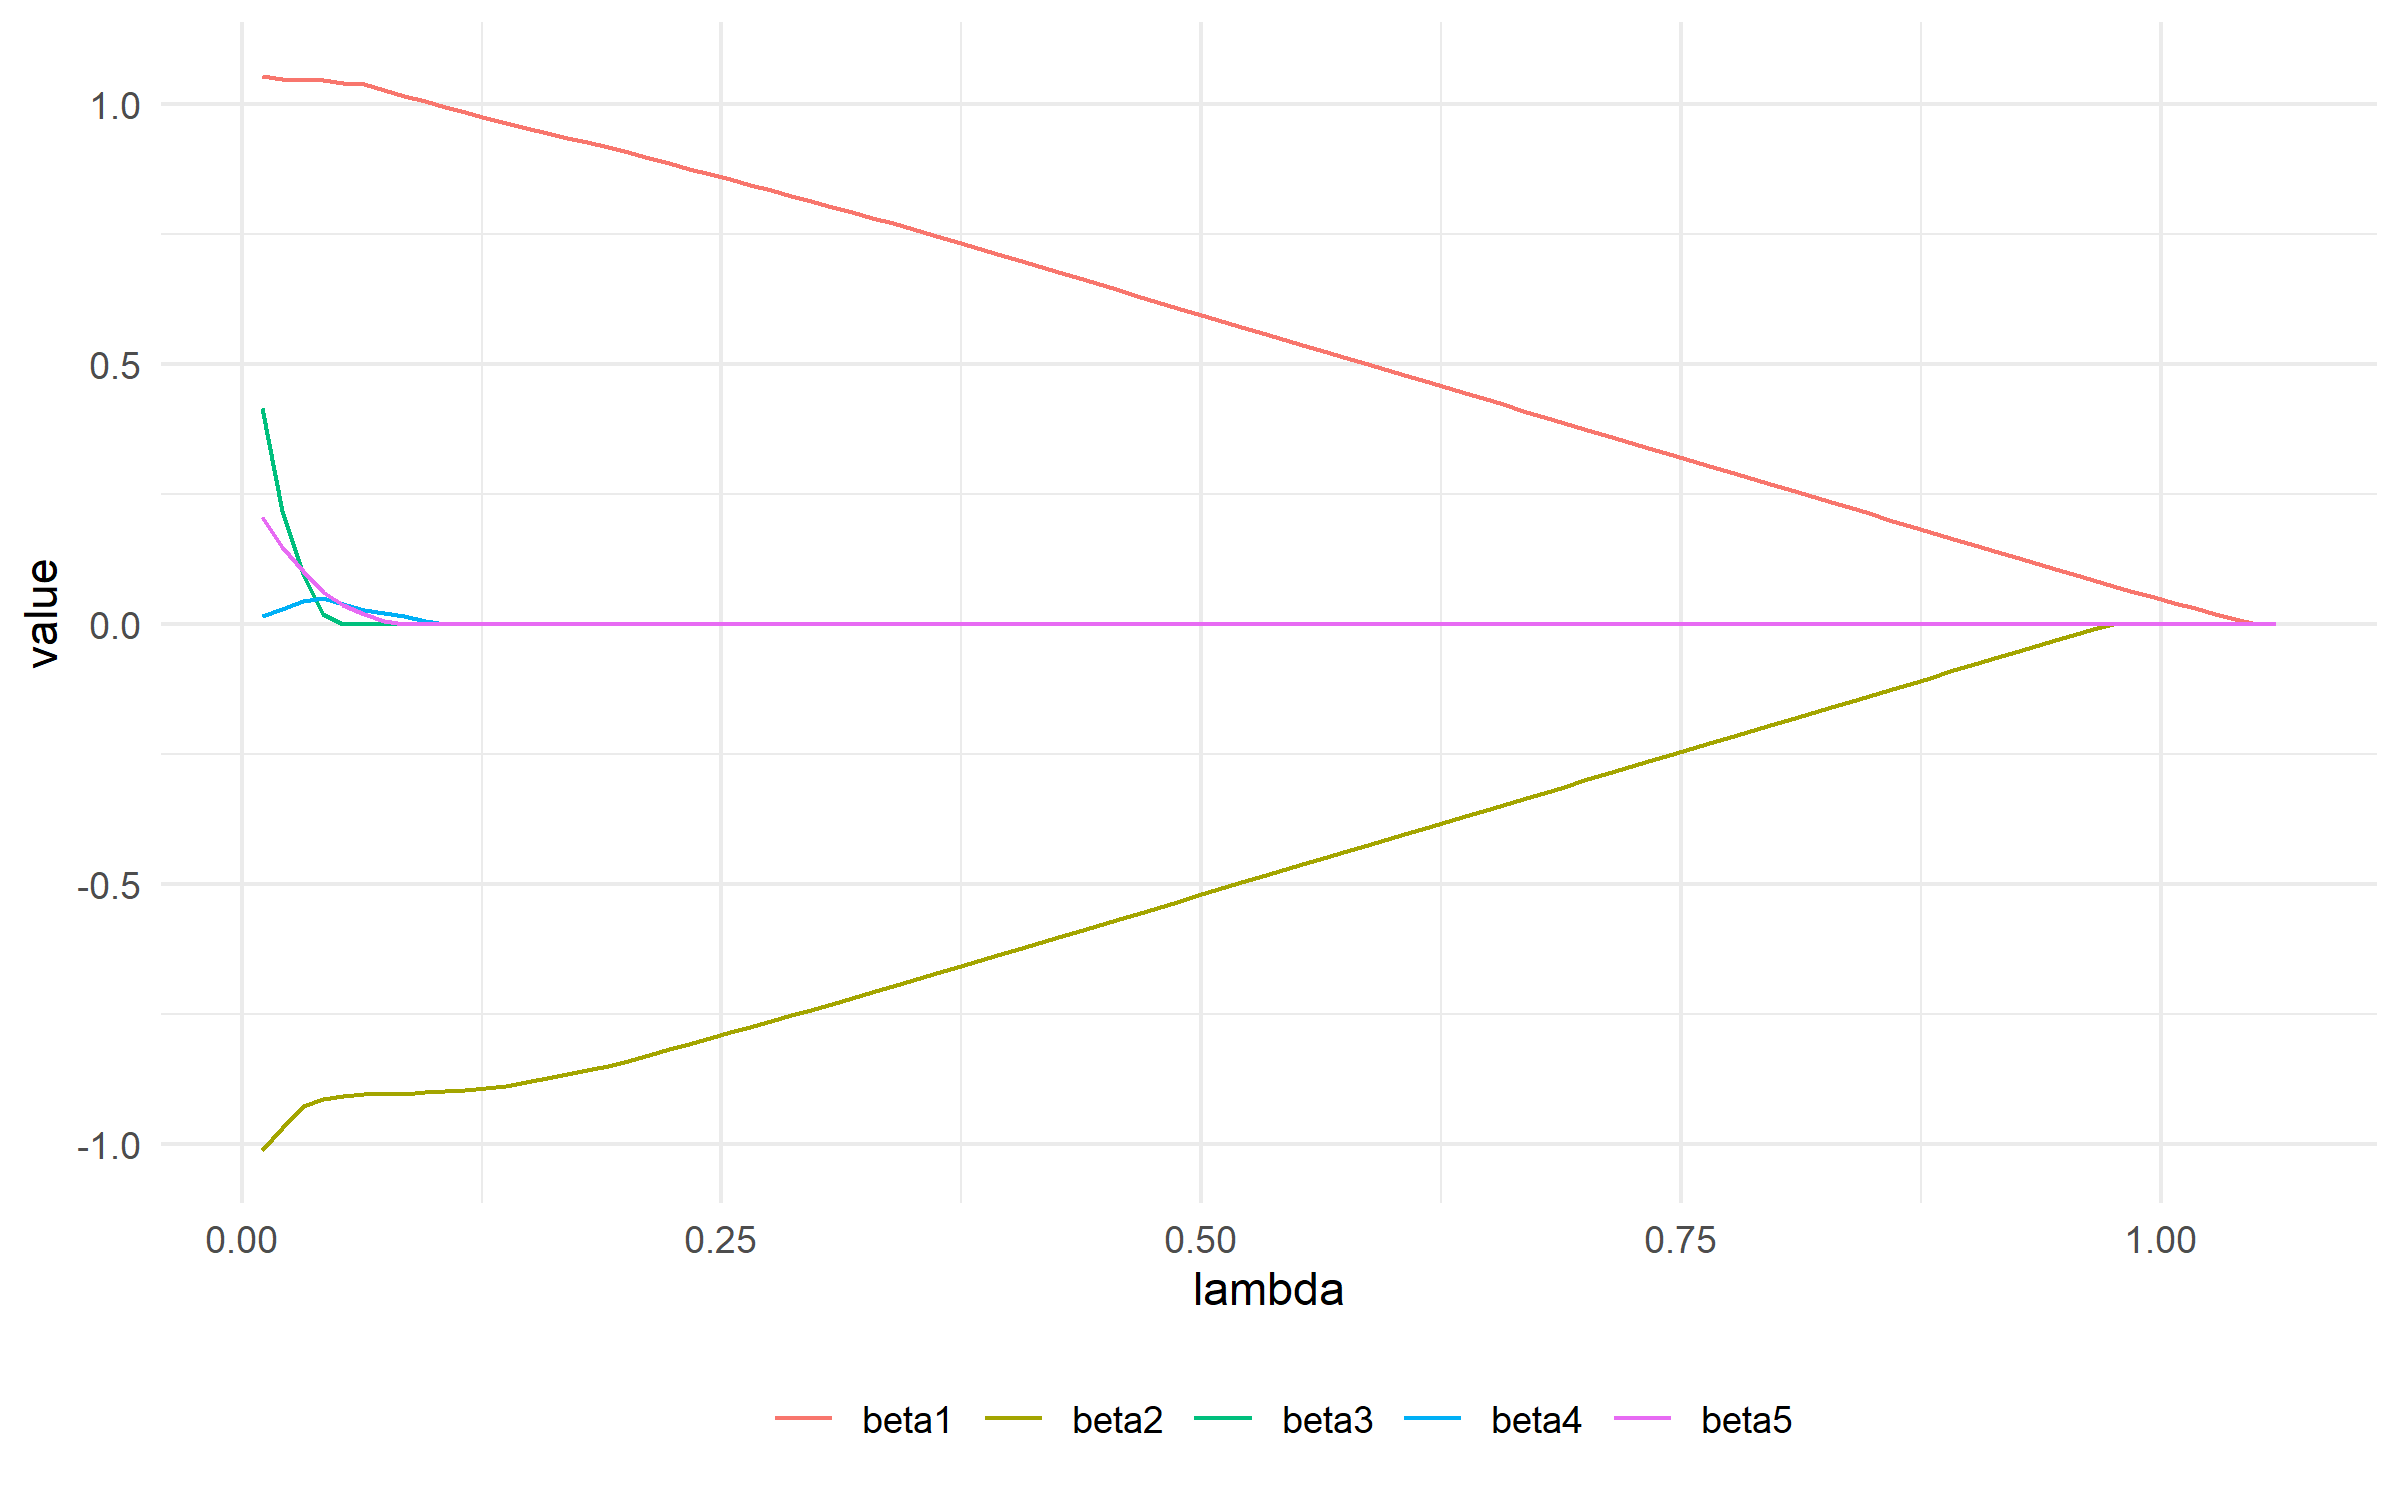
\includegraphics[width=.8\textwidth]{beta_lambdas.png}
    \caption{Value of coefficients with varying $\lambda$}
\end{figure}

\newpage
\section*{Exercise 2b}
The MSFE drops and reaches a minimum at 1.5.  
\begin{figure}[!h]
    \centering
    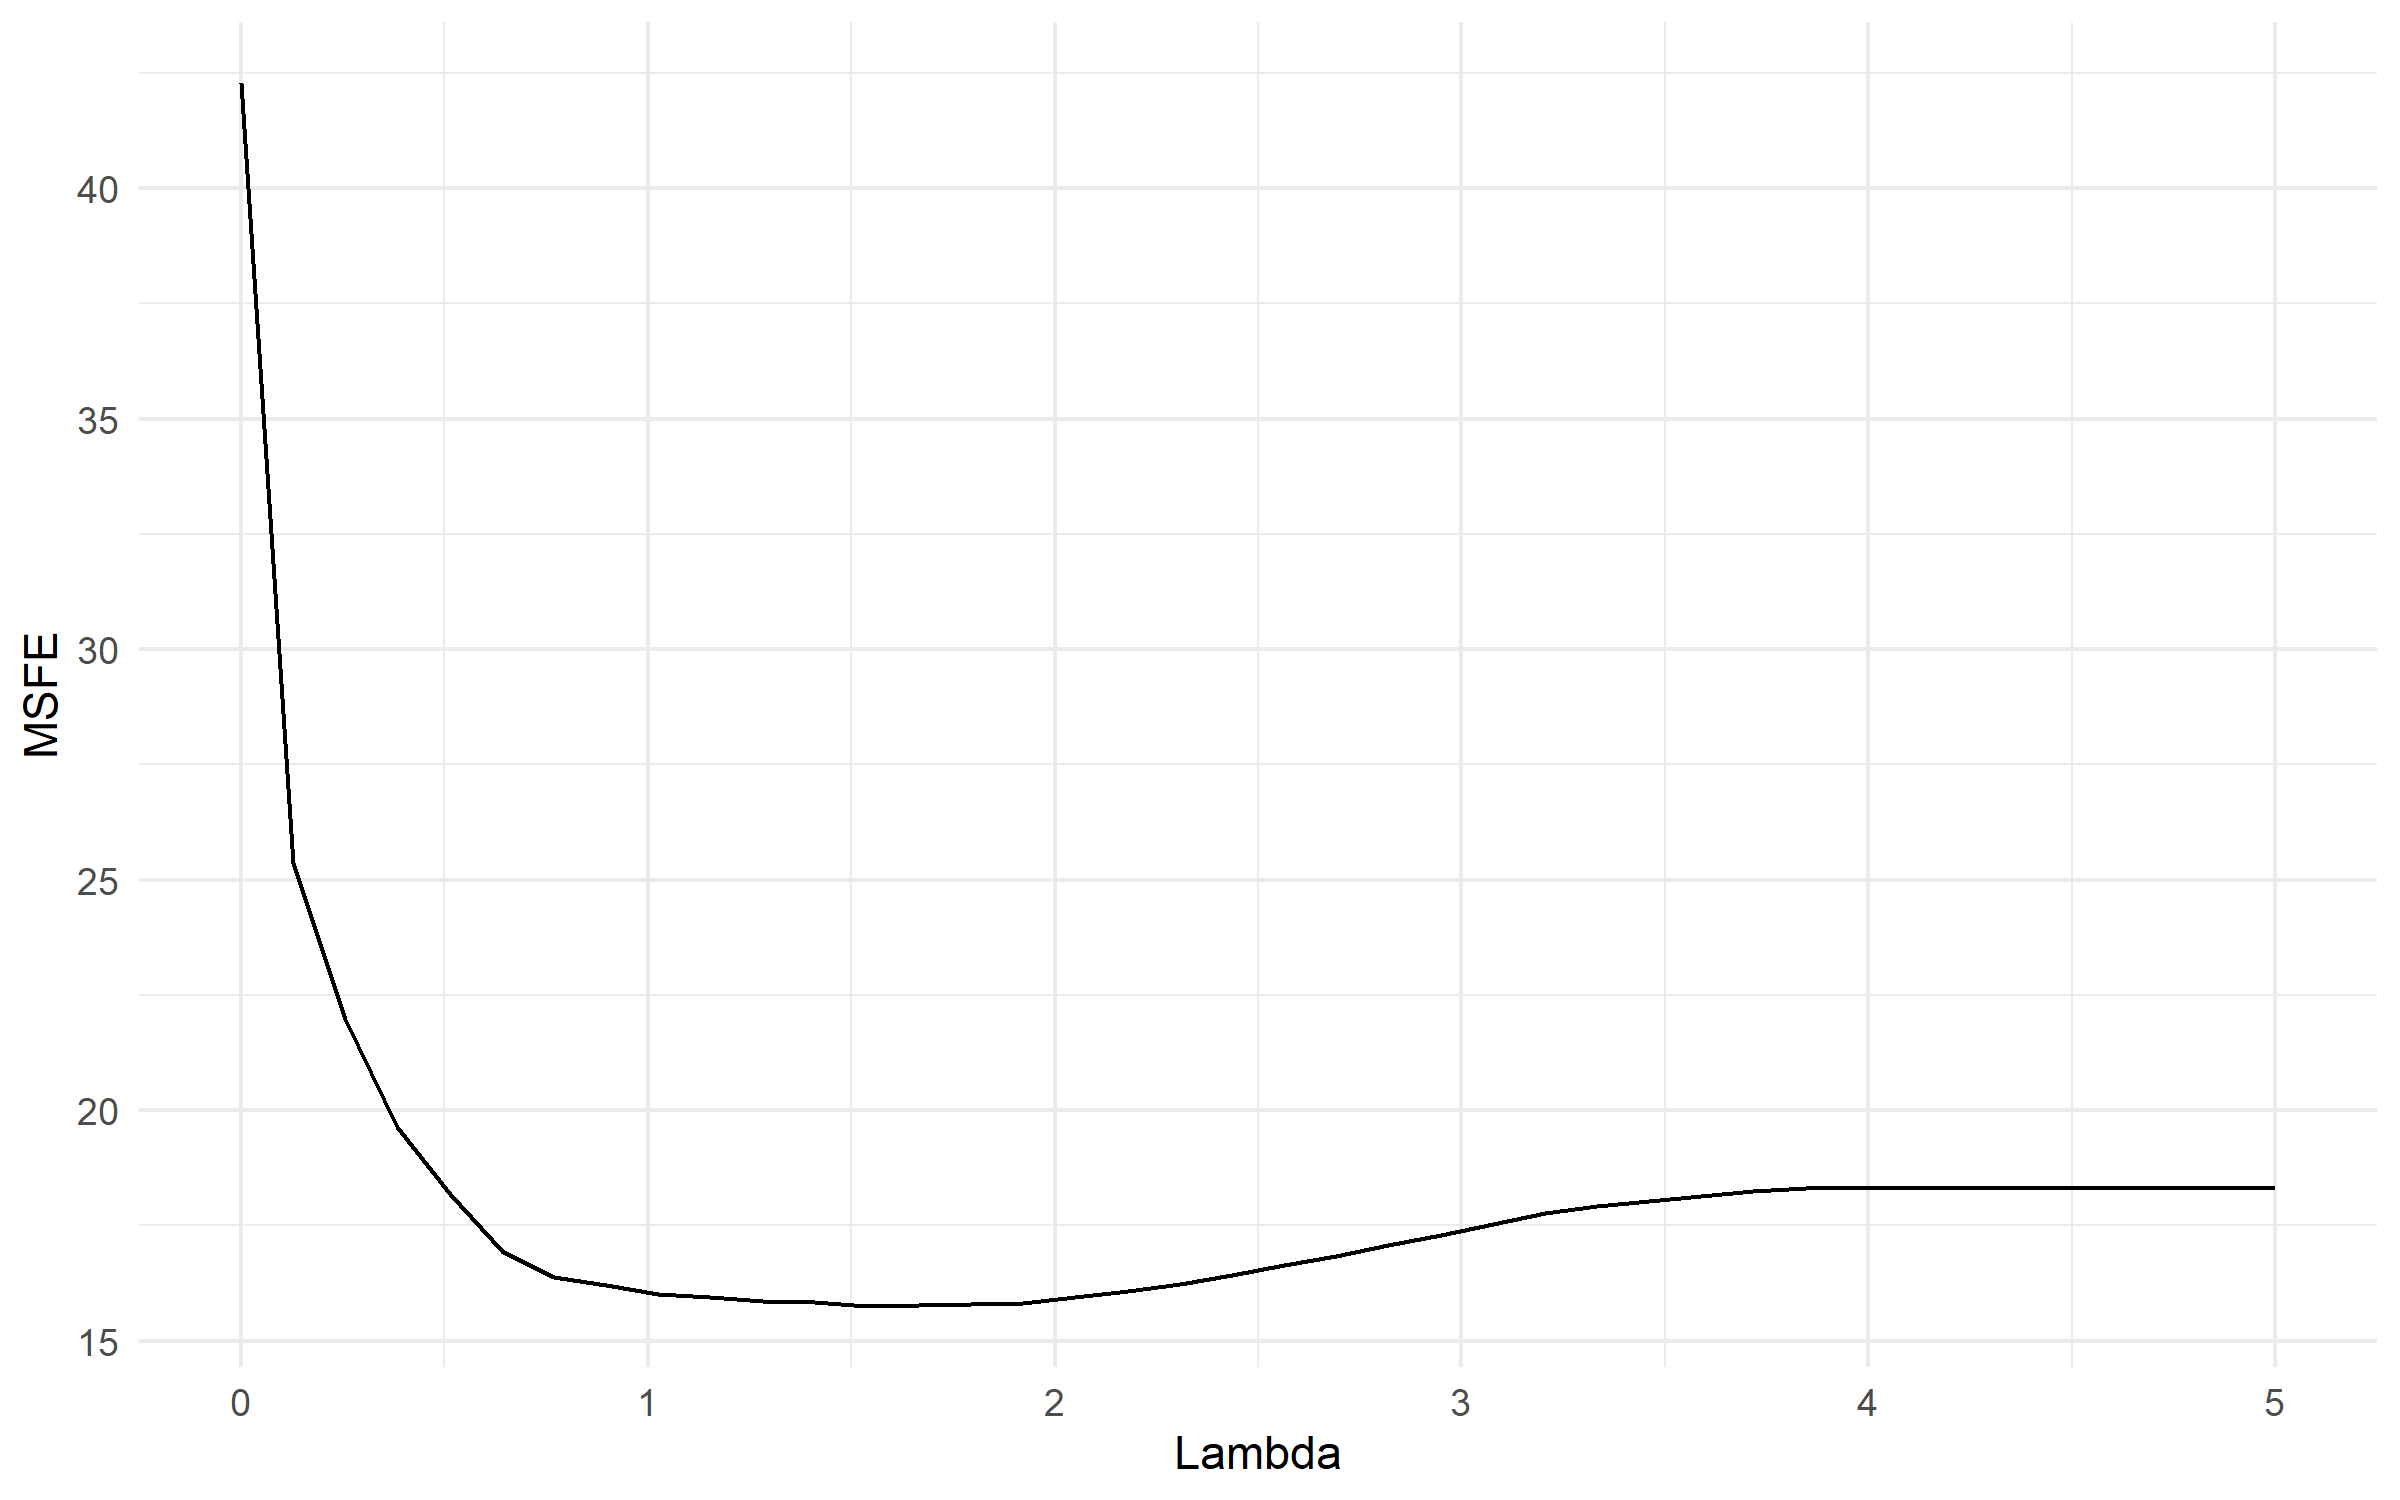
\includegraphics[width=.8\textwidth]{lambda_2b.png}
    \caption{Exercise 2b - MSFE}
\end{figure}

I report the estimates of the optimal $\lambda$ using the graph below, comparing the estimated values to the true values. We see that $\beta_1$ is biased downward, which is to be expected as we have thrown in controls that steal variation away from $\beta_1$.
\begin{figure}[!h]
    \centering
    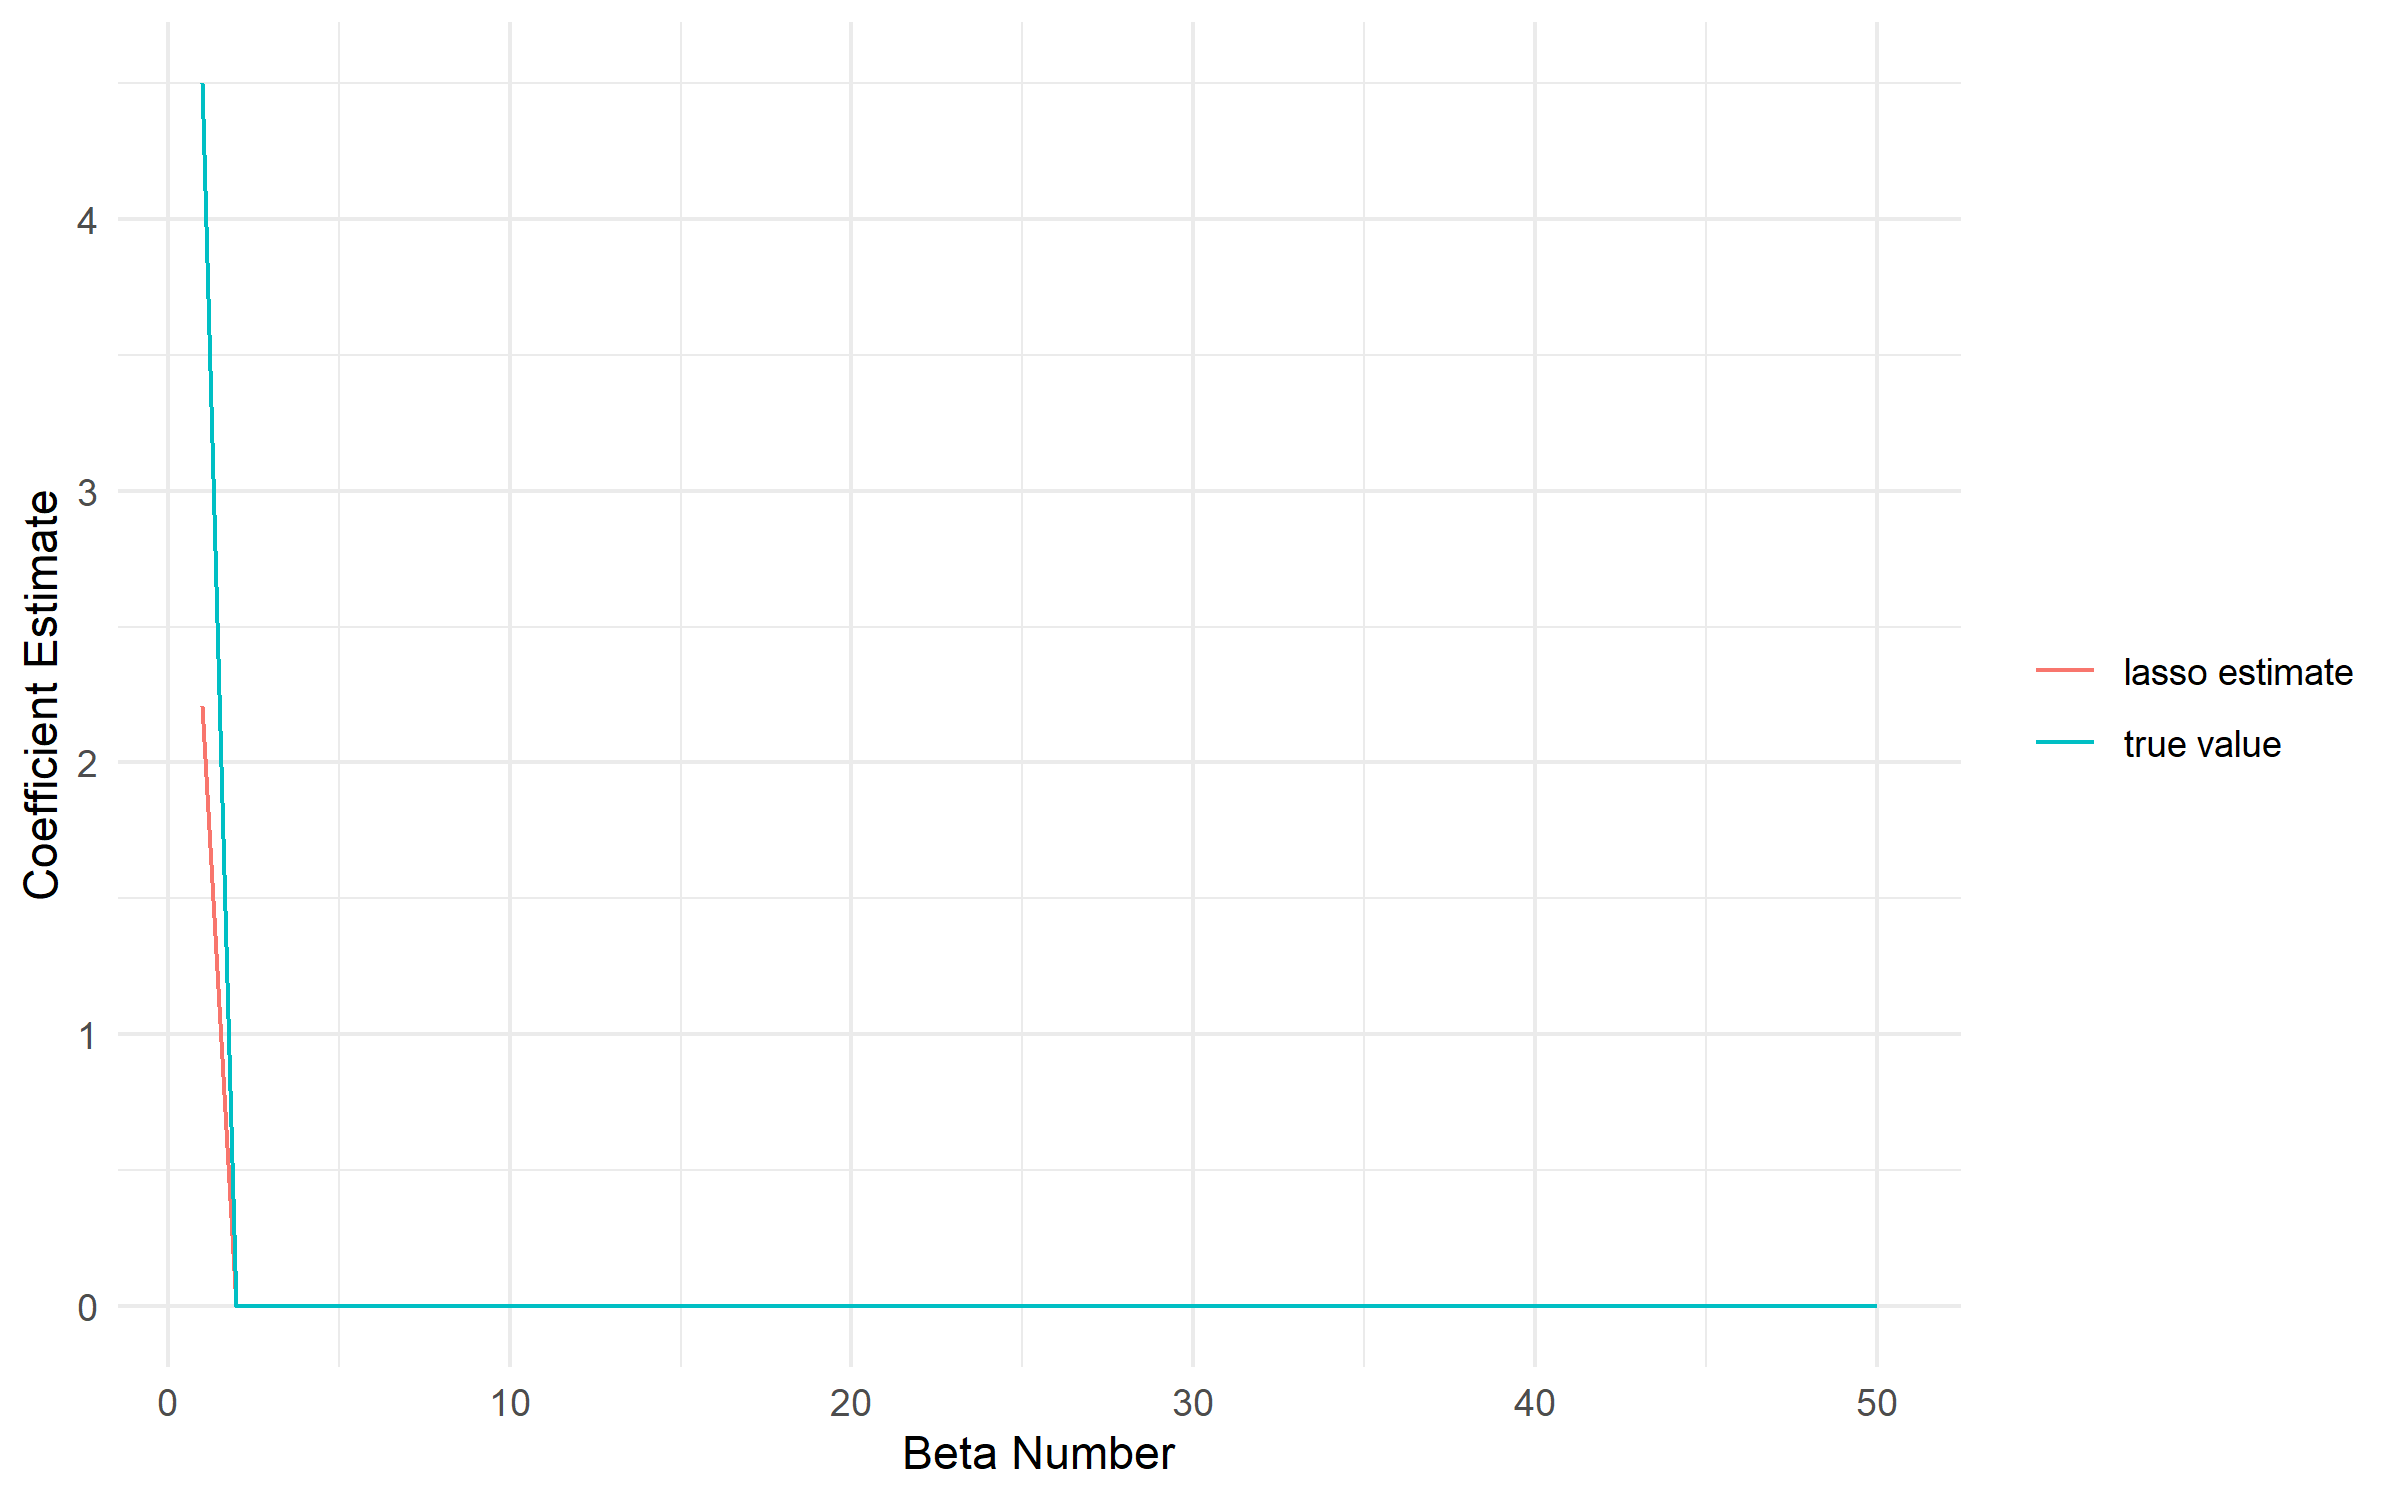
\includegraphics[width=.8\textwidth]{estimate_2b.png}
    \caption{Exercise 2b - Estimates Using Optimal $\lambda$}
\end{figure}

\section*{Exercise 2c}
We see larger values of MSFE compared to 2b. Lasso does not perform as well when there are many coefficients that are close to zero, which is the case here. 
\begin{figure}[!h]
    \centering
    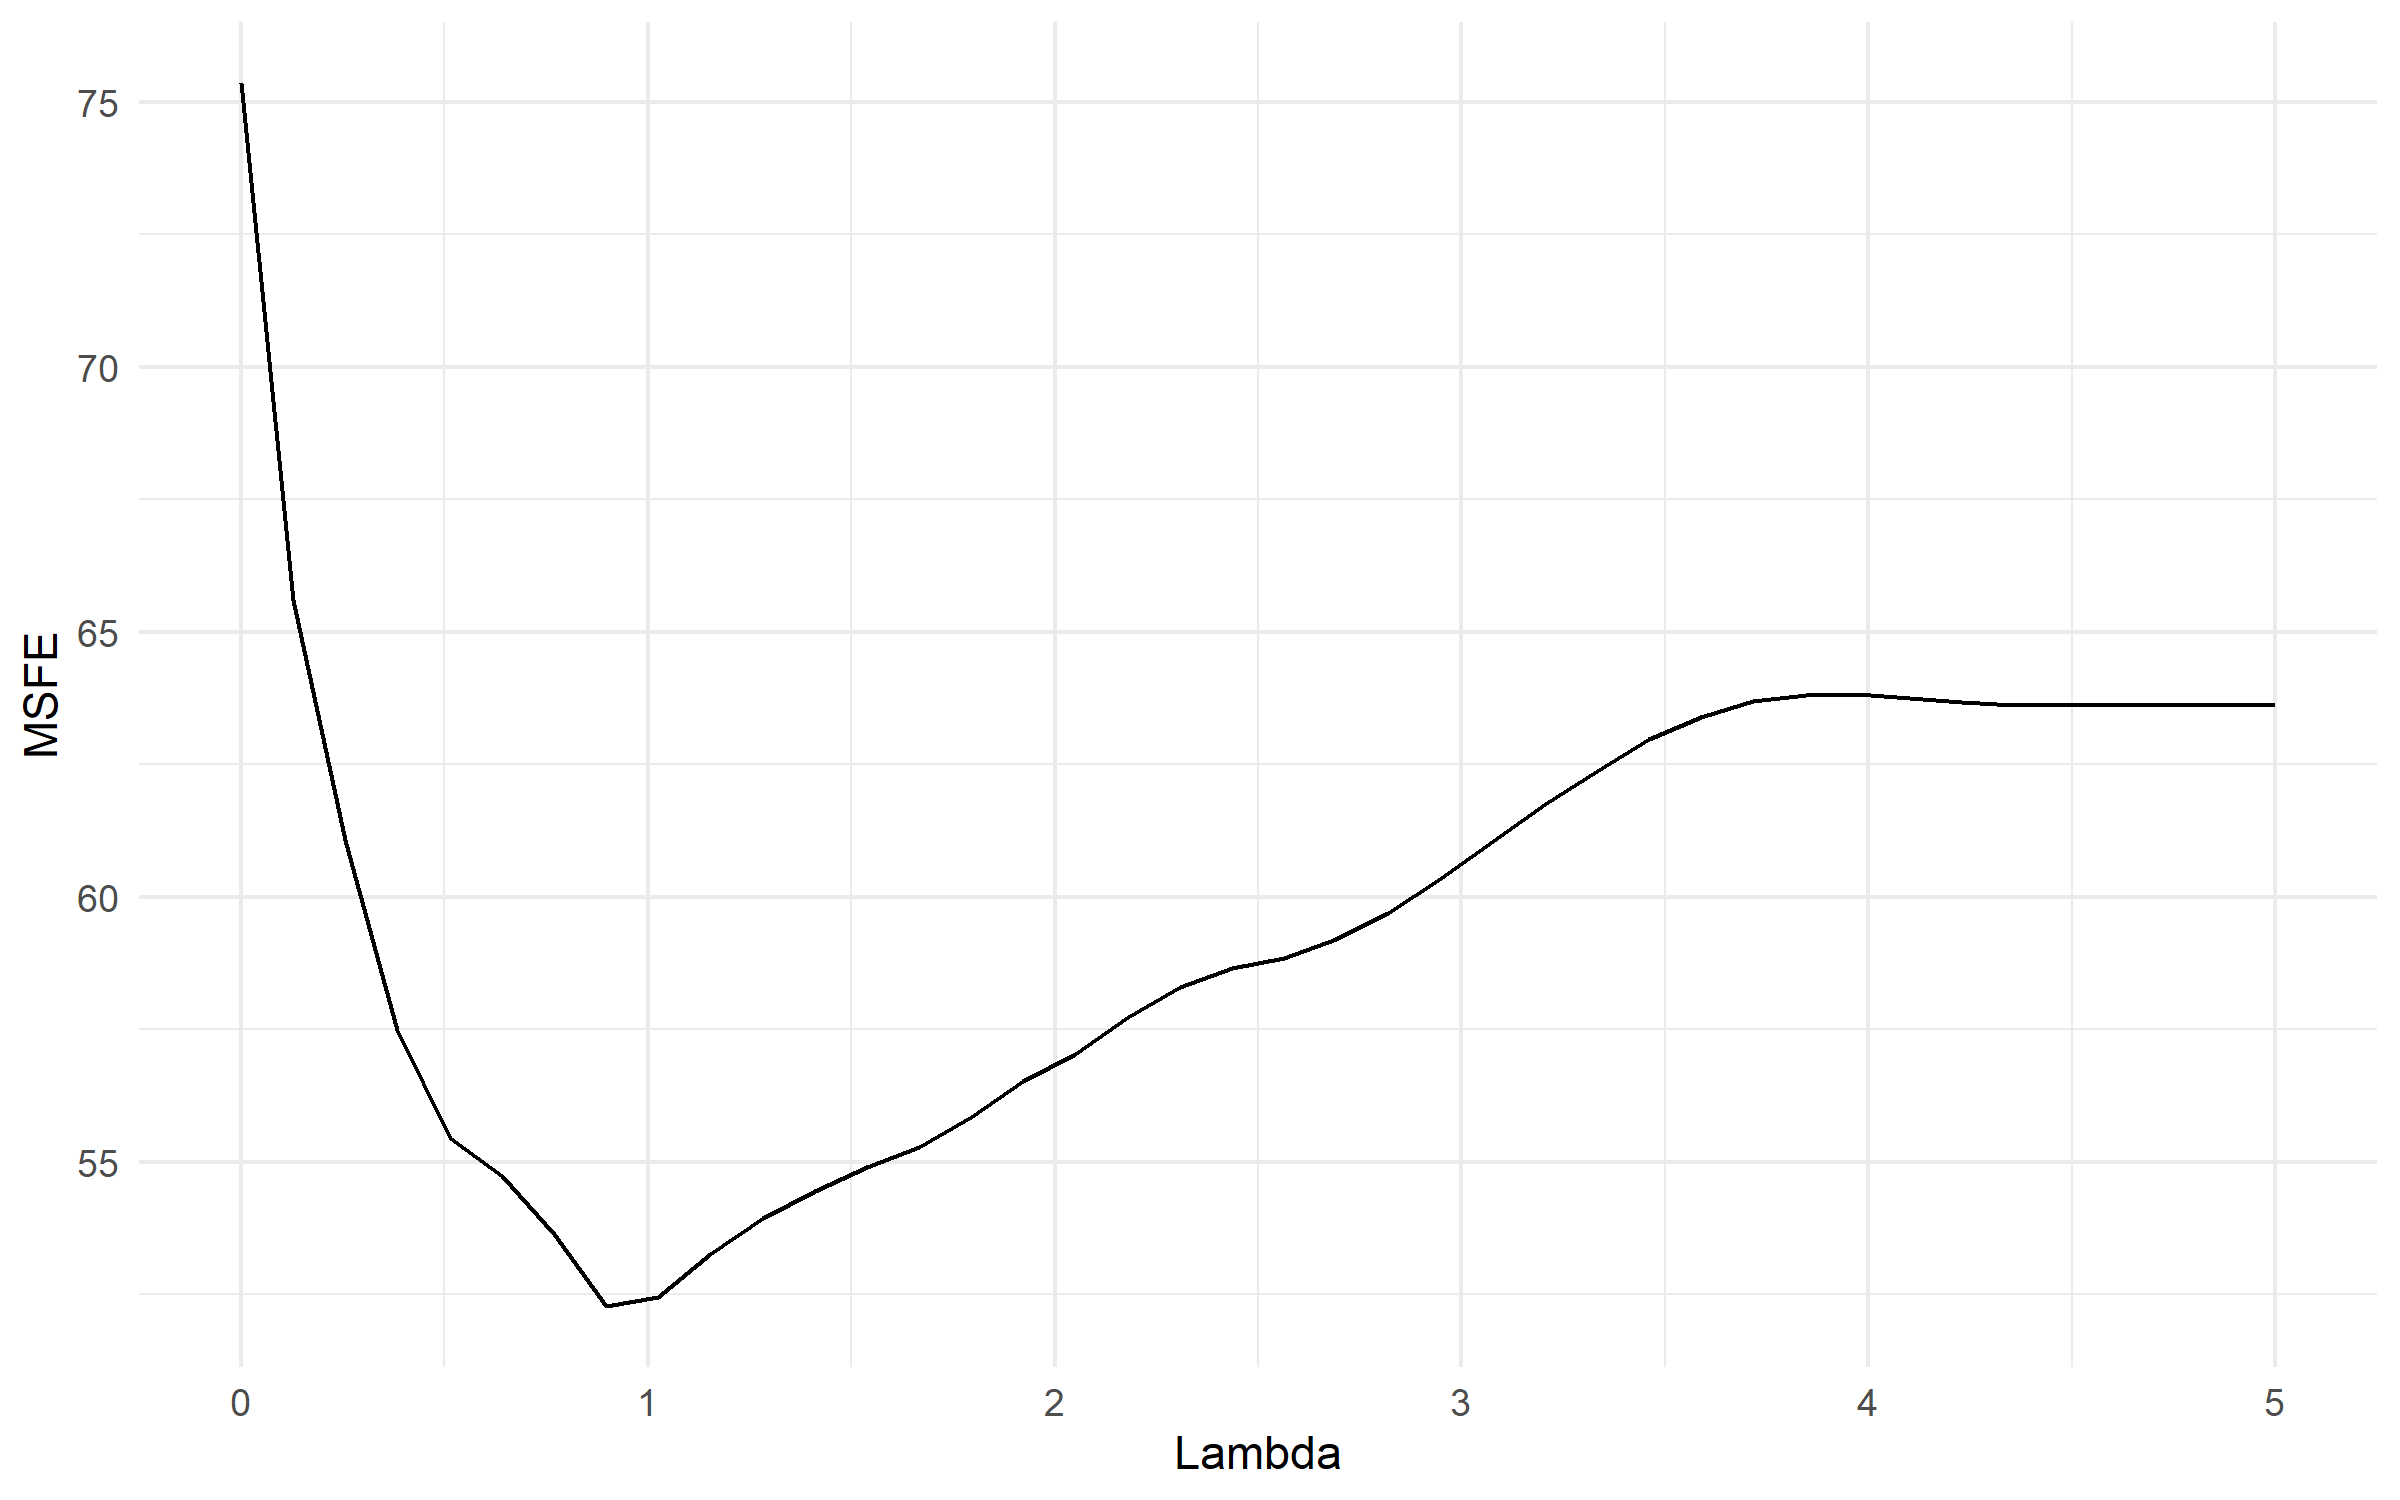
\includegraphics[width=.8\textwidth]{lambda_2c.png}
    \caption{Exercise 2c - MSFE}
\end{figure}


\begin{figure}[!h]
    \centering
    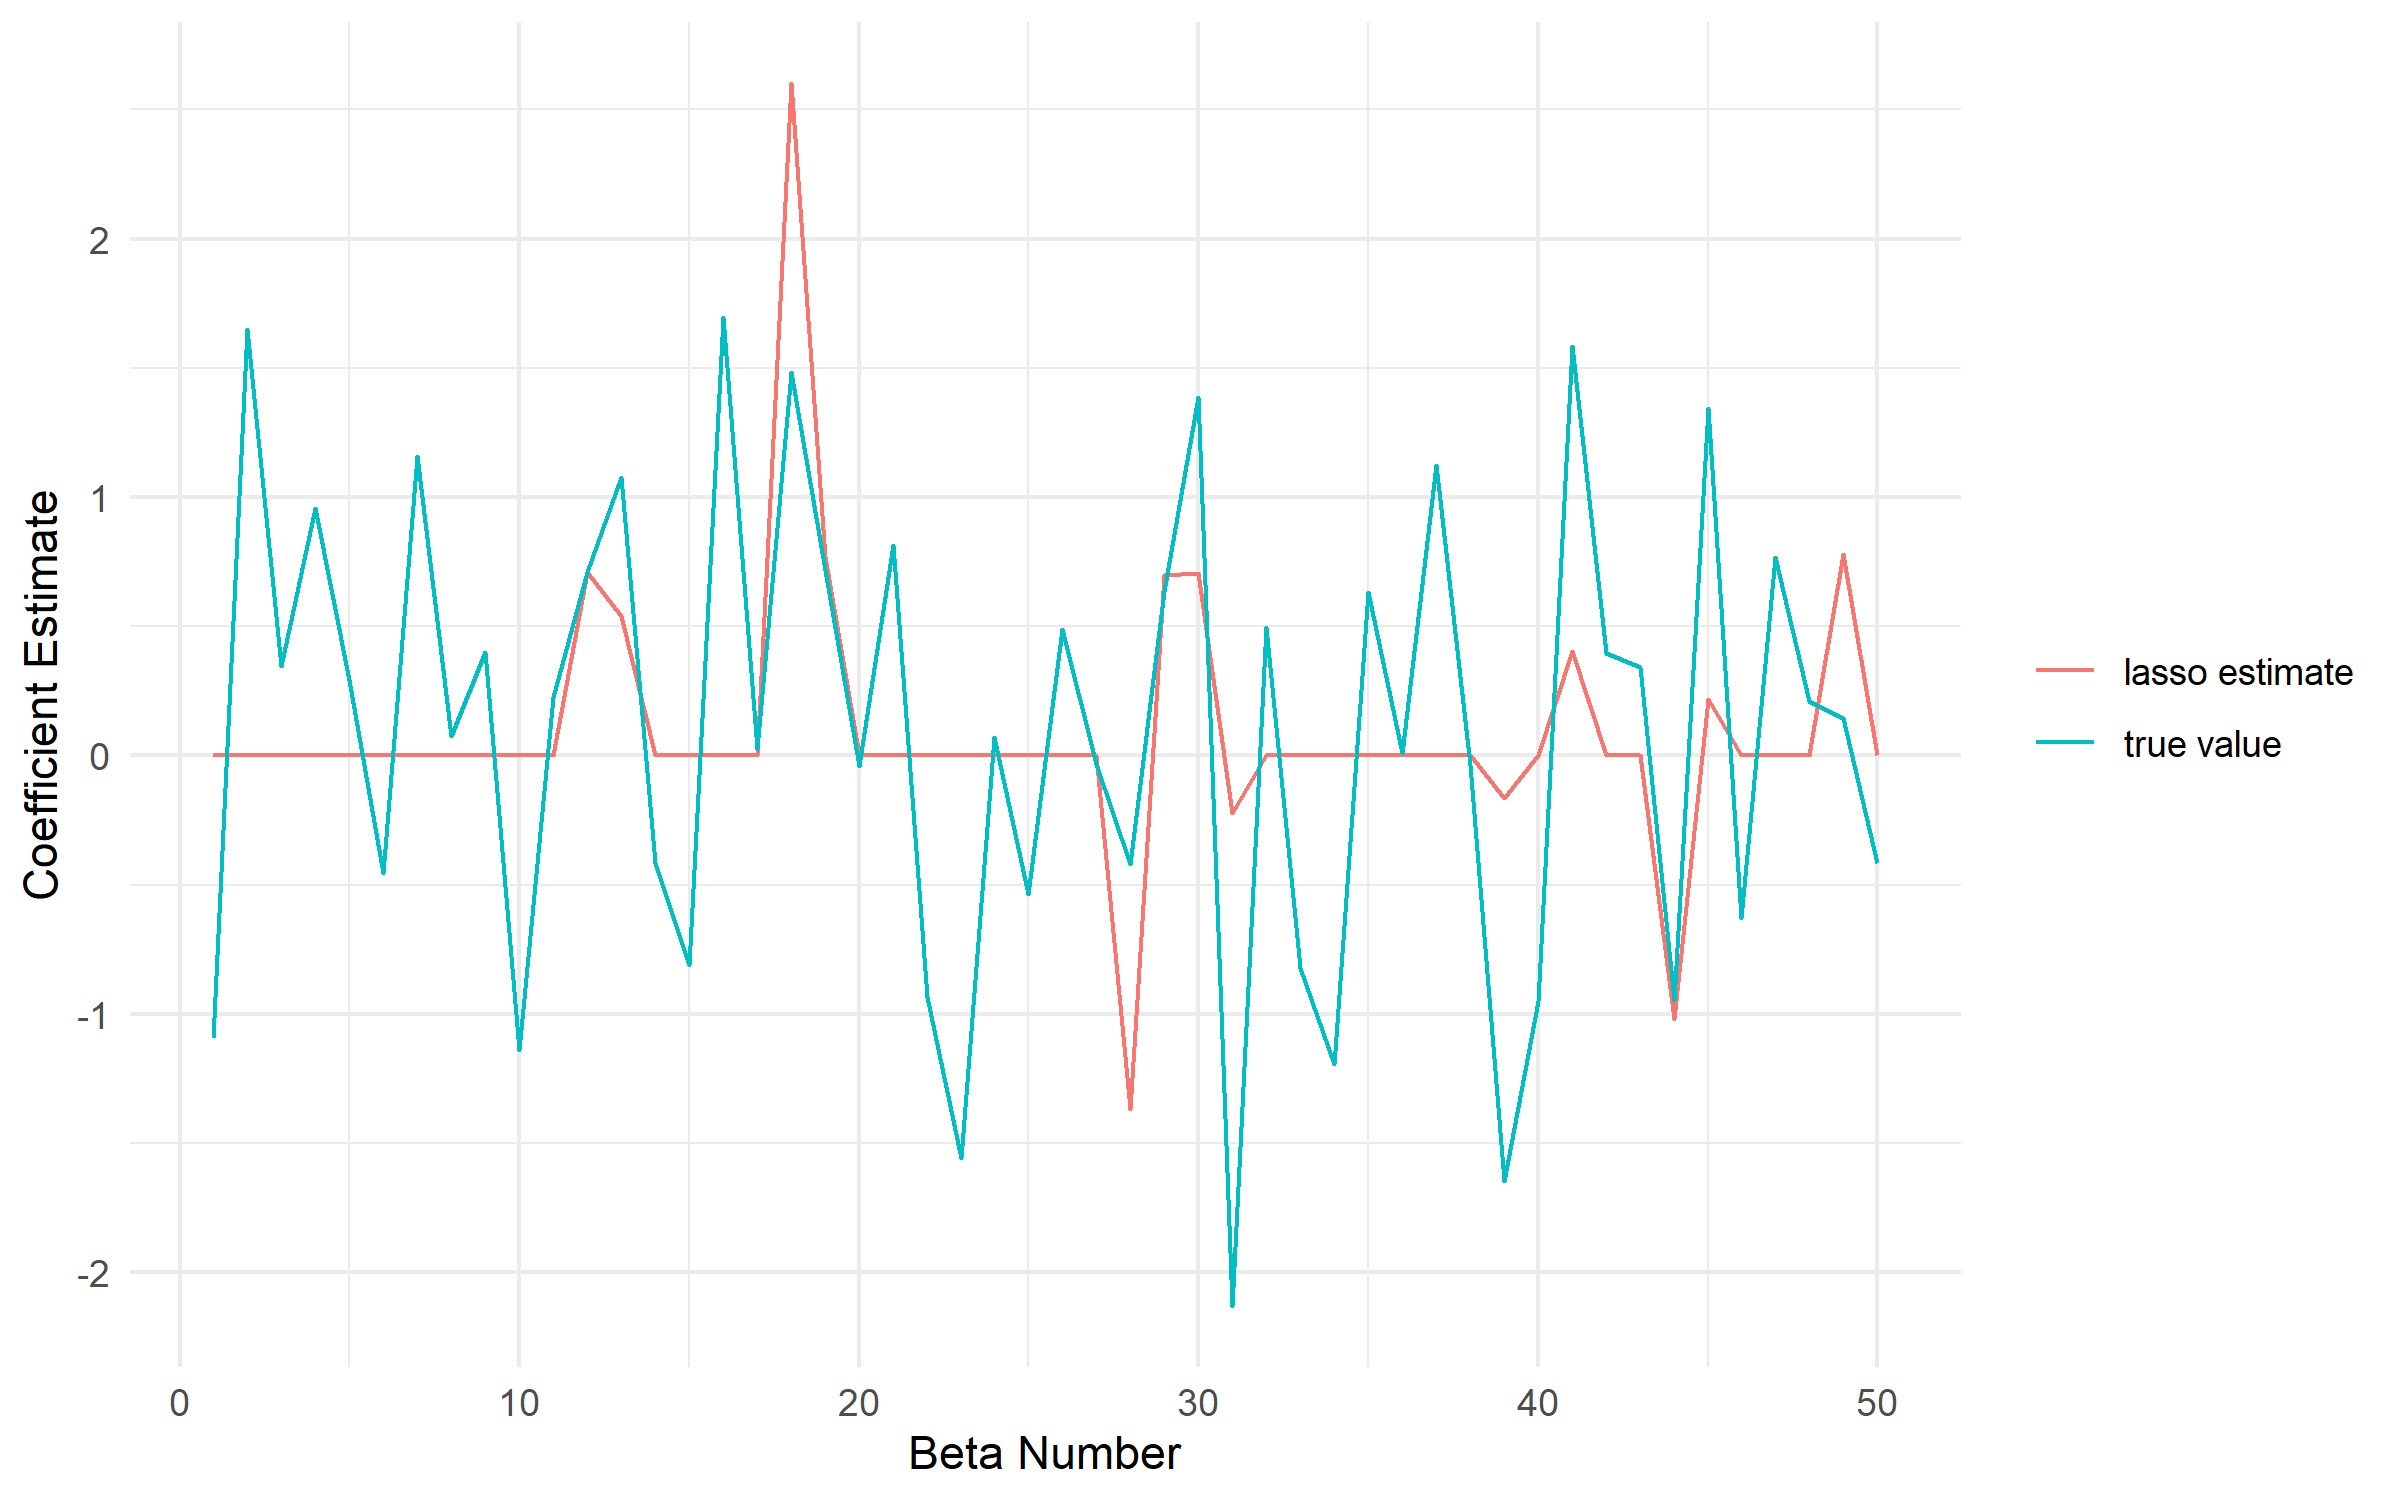
\includegraphics[width=.8\textwidth]{estimate_2c.png}
    \caption{Exercise 2c - Estimates Using Optimal $\lambda$}
\end{figure}

\newpage
\section*{Exercise 2d}
With correlation between the $X$ terms, adding all the extra $X_2...X_{90}$ terms is stealing even more variation away from $\beta_1$, so we see that the lasso estimate for $\beta_1$ is smaller and the MSFE is higher when compared to 2b. 
\begin{figure}[!h]
    \centering
    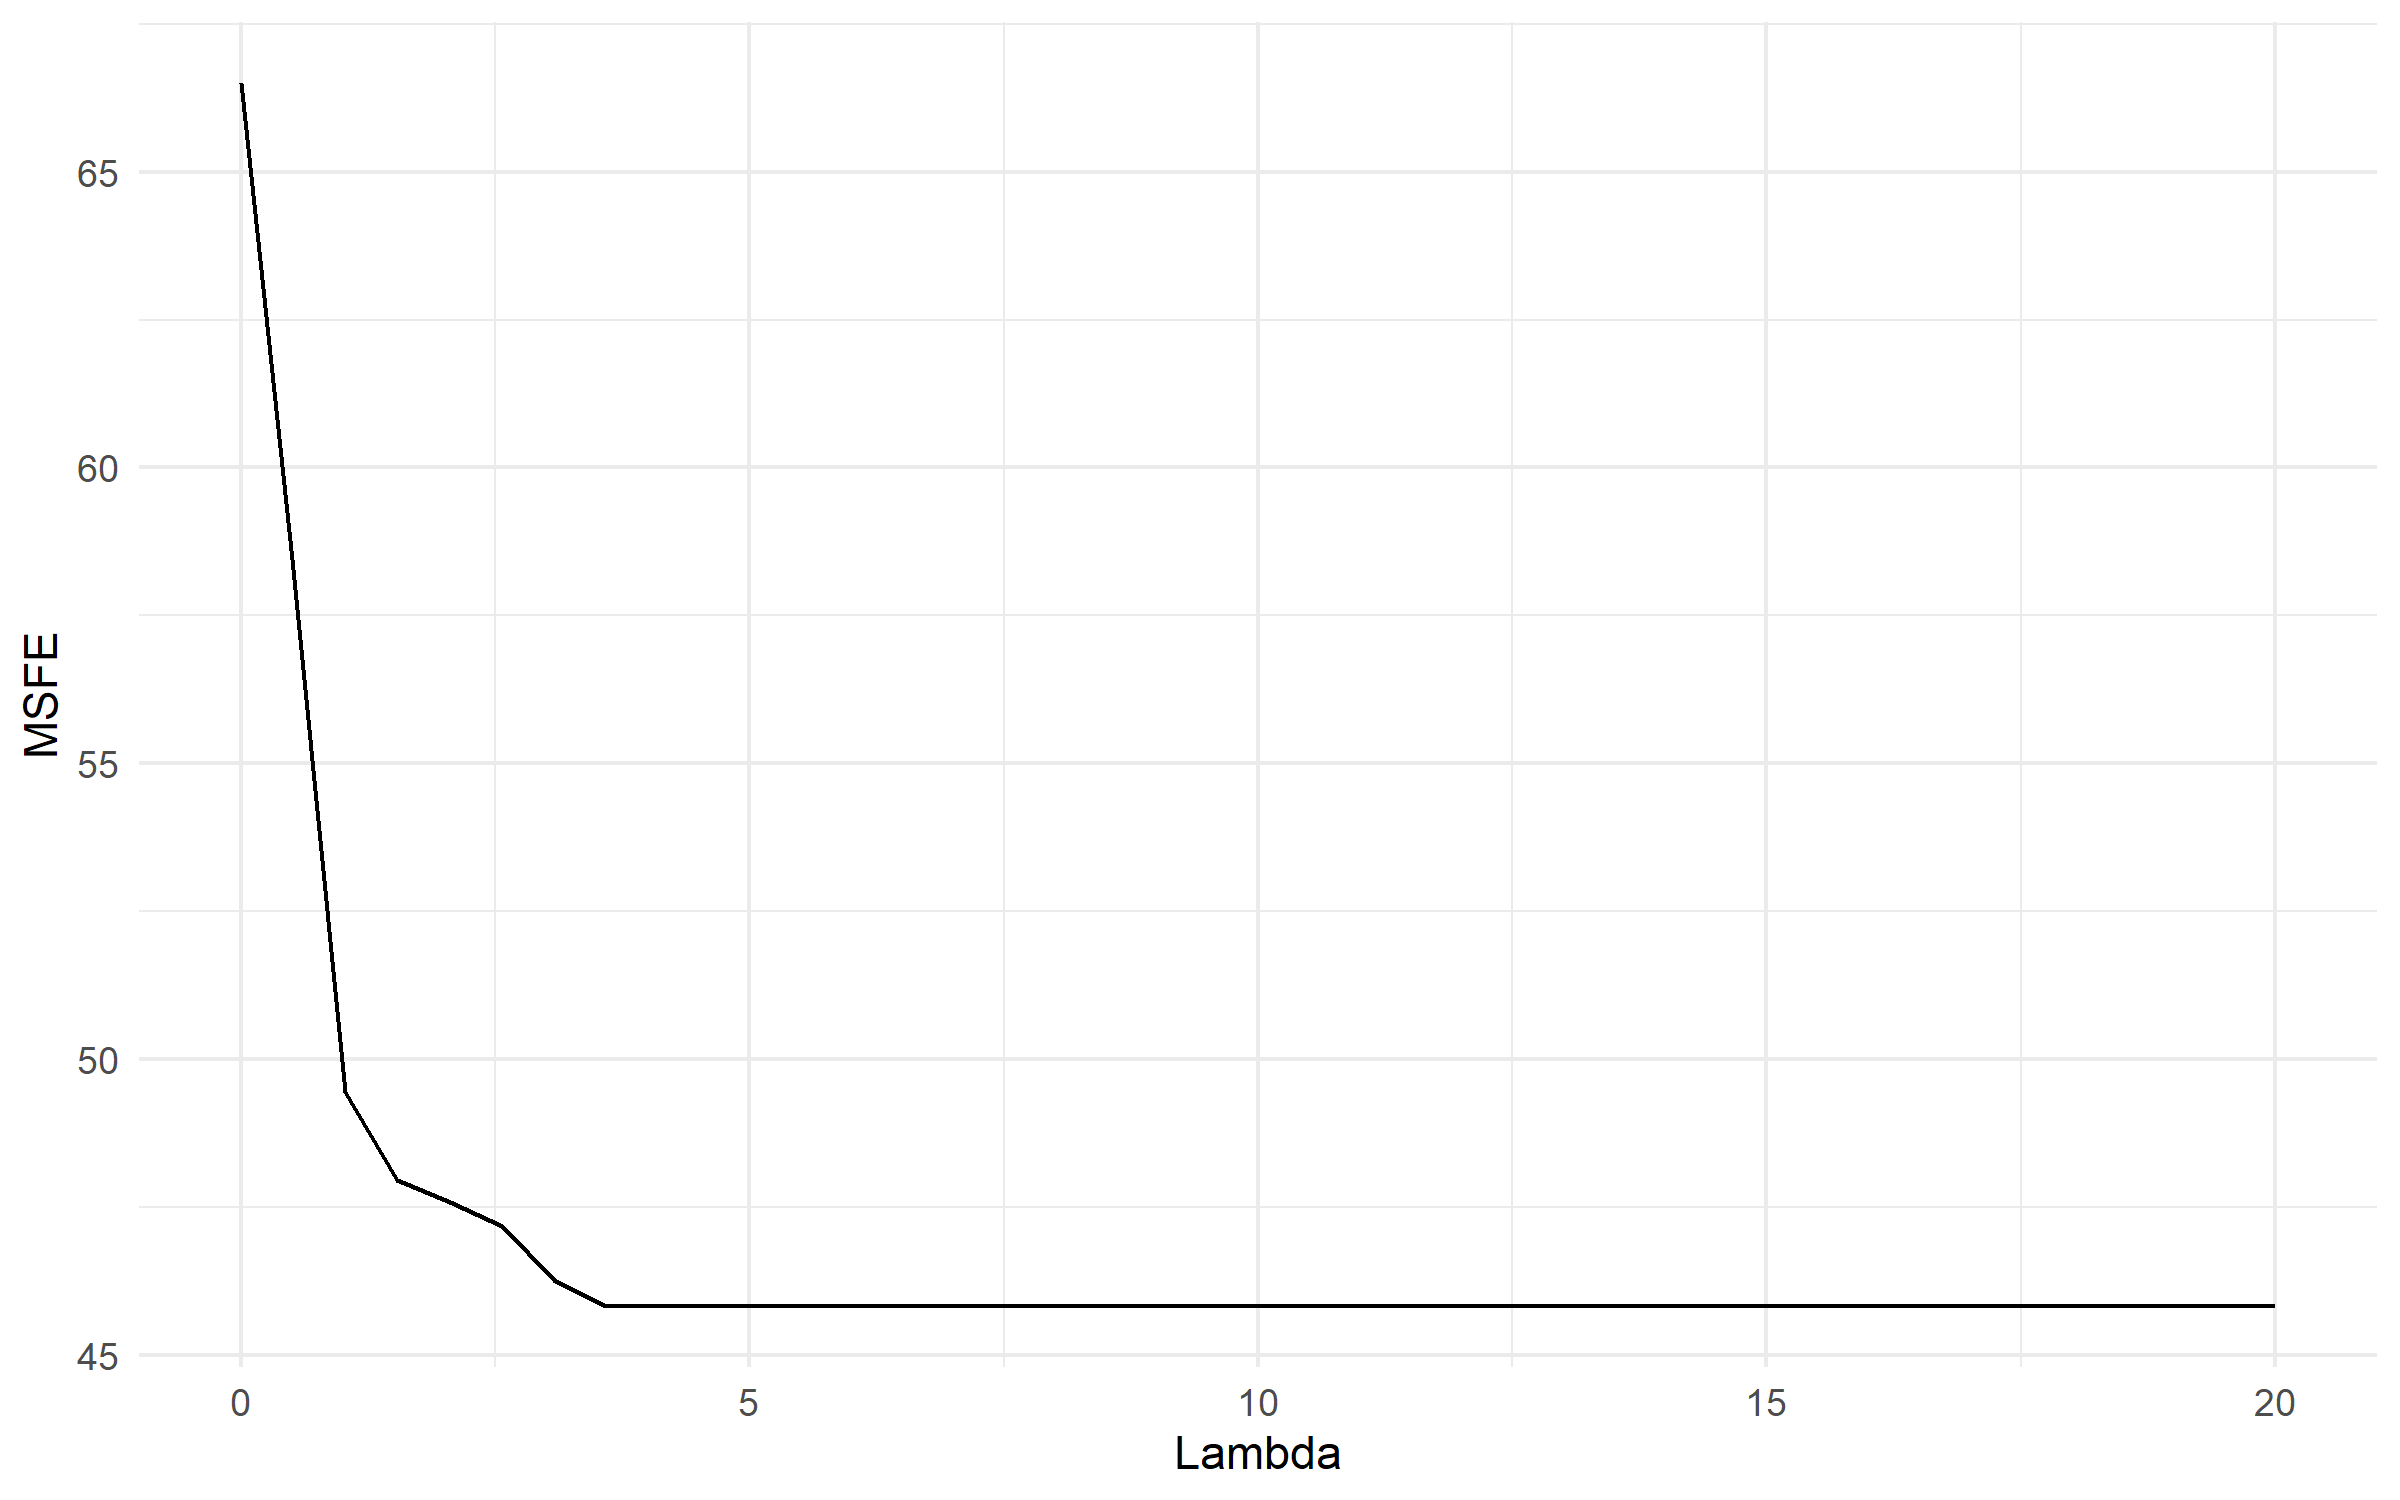
\includegraphics[width=.8\textwidth]{lambda_2d.png}
    \caption{Exercise 2d - MSFE}
\end{figure}

\begin{figure}[!h]
    \centering
    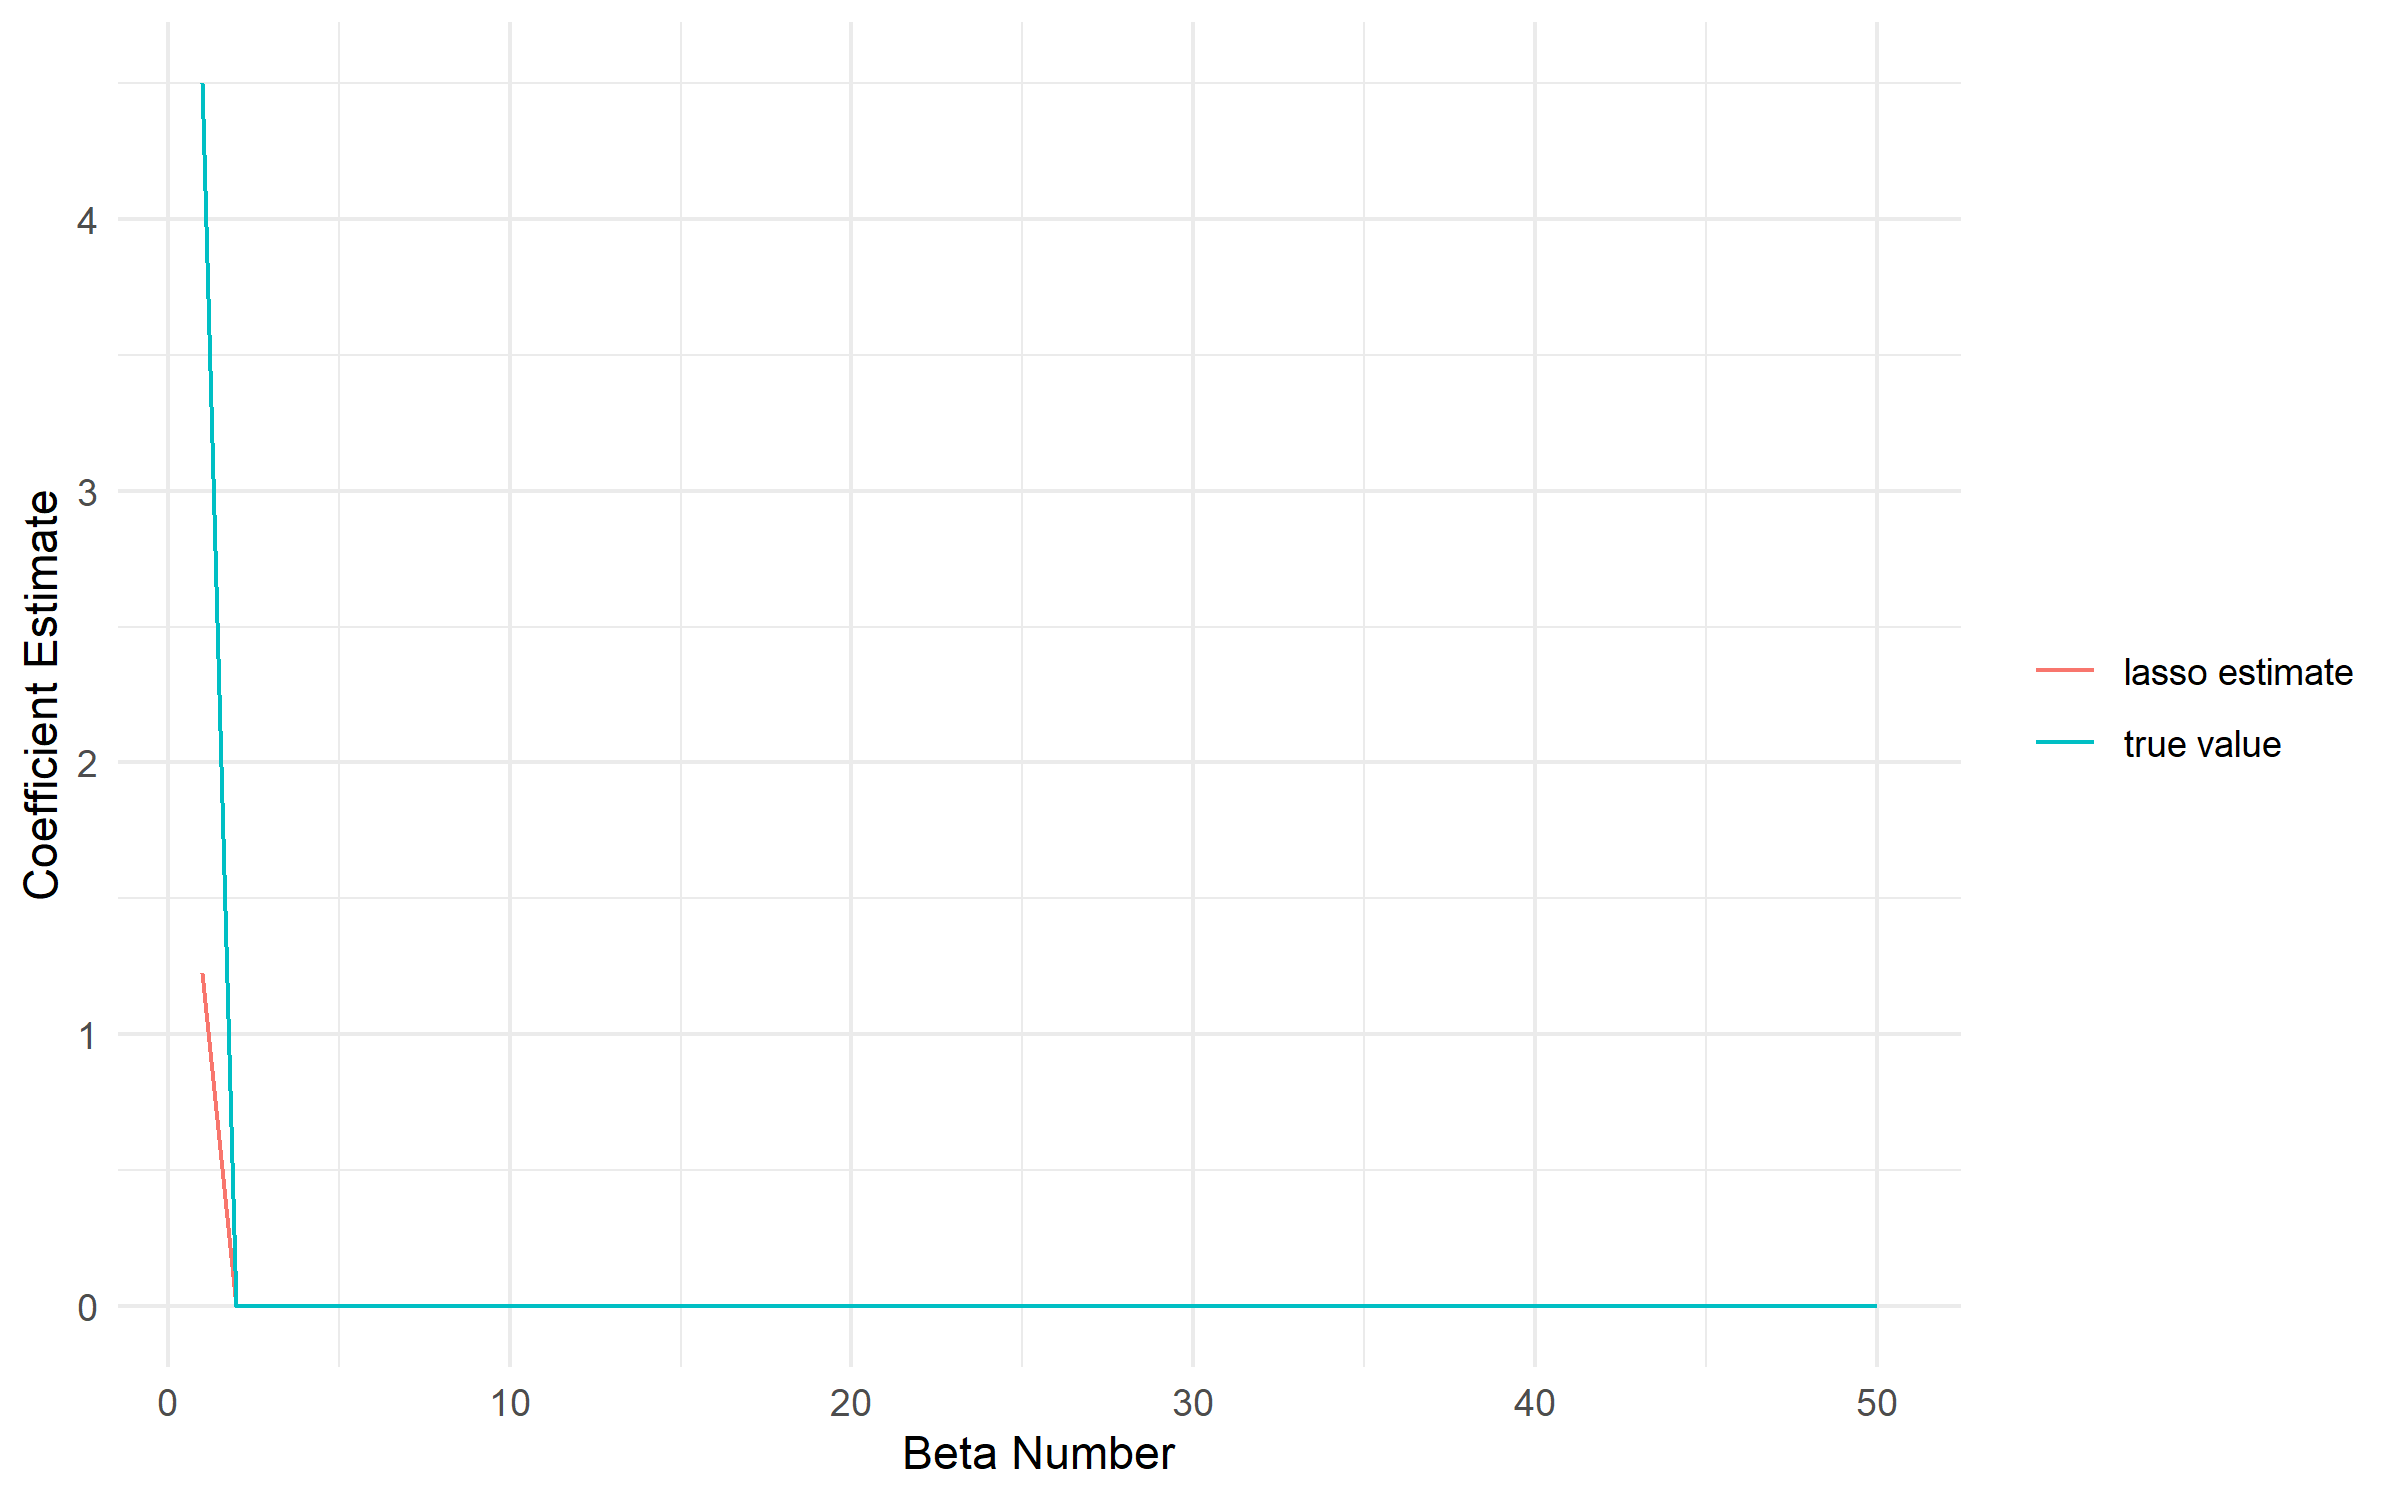
\includegraphics[width=.8\textwidth]{estimates_2d.png}
    \caption{Exercise 2d - Estimates Using Optimal $\lambda$}
\end{figure}
\end{document}
